\documentclass[conference]{IEEEtran}
\usepackage{amsmath,amssymb,graphicx,booktabs,hyperref,array}
\usepackage{tikz}
\usetikzlibrary{arrows.meta, positioning}
\usepackage[T1]{fontenc}
\usepackage{caption}
\usepackage{float}
\hypersetup{hidelinks}
\title{Half-Hop:A Graph Upsampling Approach for Slowing Down Message Passing}
\author{\IEEEauthorblockN{Tejinderpal Singh (20245161), Yuvraj Rajput (202451139), Ramswarup Swami (202451141)}
\IEEEauthorblockA{Department of Information Technology\\
Indian Institute of Information Technology, Vadodara\\
Guided by Dr. Jignesh Patel}}
\markboth{HALF-HOP: GRAPH UPSAMPLING FOR SLOWER MESSAGE PASSING}{}
\begin{document}
\maketitle
\begin{abstract}
Message-passing neural networks can suffer from over-smoothing and can be particularly sensitive to heterophilic neighborhoods. This report presents a reproduction-oriented implementation of Half-Hop, a graph upsampling method that inserts virtual slow nodes along graph edges. We evaluate GCN, GraphSAGE, and GAT with and without Half-Hop on six heterophilic node-classification benchmarks, reproduce Texas connectivity and initialization ablations, and apply the method to ModelNet10 3D mesh graph classification. The stored project results show consistent GCN gains across all six heterophilic datasets, large GAT gains on several datasets, and modest effects on ModelNet10 under a single-seed protocol.
\end{abstract}
\begin{IEEEkeywords}
graph neural networks, message passing, graph augmentation, Half-Hop, heterophily, over-smoothing, GCN, GraphSAGE, GAT
\end{IEEEkeywords}

\section{Introduction}
Graph neural networks (GNNs) learn representations by propagating information over graph edges. Repeated propagation can make node representations increasingly similar, a phenomenon commonly called over-smoothing. The problem is especially important on heterophilic graphs, where neighboring nodes are often associated with different classes and indiscriminate aggregation can mix useful and harmful information \cite{pei}.

Half-Hop \cite{azabou} addresses this issue through a graph-level intervention rather than a specialized encoder. For a directed source-to-target edge, a new intermediate slow node is inserted, creating a longer propagation path while preserving compatibility with standard message-passing architectures. The source paper reports improvements across supervised and self-supervised benchmarks, especially under heterophily.

This project implements the core operator in PyTorch Geometric, provides GCN, GraphSAGE, and GAT baselines and Half-Hop variants, stores results for six heterophilic benchmarks, reproduces Texas ablations, and evaluates the method on ModelNet10 3D mesh graph classification. This report focuses on the computational workflow and implementation architecture of the reproduced method. Our objective is a software reproduction that makes the pipeline understandable, runnable, and testable from end-to-end.

\section{Related Work and Paper Analysis}
The source paper \cite{azabou} presents Half-Hop as graph upsampling analogous to increasing image resolution. Instead of adding pixels, it adds nodes along graph edges and interpolates their features. The transformed graph is then passed to a conventional message-passing network without changing the encoder or loss.

Its analysis studies receptive fields and message-passing dynamics. A direct one-hop interaction becomes a two-step route through a slow node, reducing the speed at which neighborhood information reaches a node. The theoretical treatment connects this slower smoothing to preservation of small spectral components and delayed over-smoothing. The paper evaluates GCN \cite{kipf}, GraphSAGE \cite{hamilton}, and GAT \cite{gat} and also uses Half-Hop as an augmentation for BGRL \cite{thakoor}.

\section{Methodology}
\subsection{Half-Hop transformation}
For a directed edge $e_{ij}$, the proposed transformation introduces a slow node $\nu_k$ and uses
\begin{equation}
v_i \rightarrow \nu_k \leftrightarrow v_j.
\end{equation}
Both endpoints send information to the slow node, while the slow node sends information toward the original target. Self-loops are preserved and are not half-hopped.

\begin{figure}[H]
\centering
\resizebox{\columnwidth}{!}{%
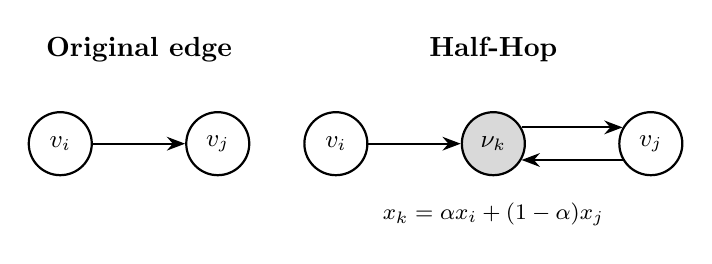
\begin{tikzpicture}[
    main node/.style={circle, draw, minimum size=0.8cm, font=\small, thick},
    slow node/.style={circle, draw, fill=gray!30, minimum size=0.8cm, font=\small, thick},
    >=Stealth,
    thick
]
    % Original edge
    \node (orig_title) at (0, 1.2) {\textbf{Original edge}};
    \node[main node] (vi) at (-1, 0) {$v_i$};
    \node[main node] (vj) at (1, 0) {$v_j$};
    \draw[->] (vi) -- (vj);

    % Half-Hop
    \node (hh_title) at (4.5, 1.2) {\textbf{Half-Hop}};
    \node[main node] (vi2) at (2.5, 0) {$v_i$};
    \node[slow node] (vk) at (4.5, 0) {$\nu_k$};
    \node[main node] (vj2) at (6.5, 0) {$v_j$};
    
    \draw[->] (vi2) -- (vk);
    \draw[->] (vk.30) -- (vj2.150);
    \draw[<-] (vk.330) -- (vj2.210);
    
    \node[font=\footnotesize] at (4.5, -0.9) {$x_k = \alpha x_i + (1-\alpha) x_j$};
\end{tikzpicture}%
}
\caption{Half-Hop inserts a slow node between adjacent nodes.}
\label{fig:schematic}
\end{figure}

\subsection{Feature initialization and sampling}
The default slow-node feature is
\begin{equation}
x_k=\alpha x_i+(1-\alpha)x_j.
\end{equation}
The implementation also supports zero and random initialization. When $p<1$, target nodes are sampled and all their incoming edges are half-hopped; this is node-level rather than independent edge-level sampling.

\subsection{Integration with GNNs}
The transformed graph is processed by GCN \cite{kipf}, GraphSAGE \cite{hamilton}, or GAT \cite{gat}. Slow nodes are added as a pre-processing step by concatenating their initial features to the original node feature matrix and appending the new connections to the edge index. After message passing, the slow nodes are not explicitly removed from the graph structure; instead, a boolean slow-node mask is applied to filter out their embeddings. This ensures that only original-node embeddings are returned for the final supervised prediction and loss calculation, making Half-Hop a plug-and-play augmentation \cite{azabou}.

\section{Implementation Architecture}
\subsection{Core Augmentation Transform}
In PyTorch Geometric, the Half-Hop augmentation is implemented as a callable transform class. Rather than modifying the graph topology on the fly inside the network forward pass, the transformation is a pre-processing step. The transform isolates self-loops (which are never half-hopped), dynamically calculates the required number of slow nodes based on the target sampling probability $p$, and initializes new features. The generated graph appends the slow-node features to the original node matrix $X$ and builds the augmented adjacency matrix based on the selected connectivity scheme.

\subsection{End-to-End Pipeline}
The software pipeline strictly decouples graph augmentation from model architecture. The transformed graph is passed intact into standard PyTorch Geometric models (GCN, GraphSAGE, GAT). This design choice matters for reproducibility: it avoids rewriting GNN internals. After the message-passing layers compute the final node embeddings, the pipeline uses a stored Boolean tensor, \texttt{slow\_node\_mask}, to drop the synthetic slow nodes before the loss calculation. This ensures the output dimensions always match the original graph's node count.

\begin{figure}[H]
\centering
\resizebox{\columnwidth}{!}{%
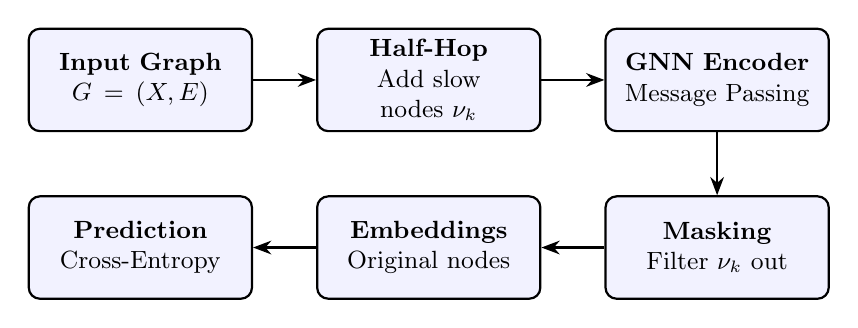
\begin{tikzpicture}[
    node distance=0.8cm and 0.8cm,
    block/.style={rectangle, draw, rounded corners, fill=blue!5, text width=2.6cm, text centered, minimum height=1.3cm, font=\small, thick},
    arrow/.style={thick, ->, >=Stealth}
]
    \node[block] (input) {\textbf{Input Graph} \\ $G = (X, E)$};
    \node[block, right=of input] (transform) {\textbf{Half-Hop} \\ Add slow nodes $\nu_k$};
    \node[block, right=of transform] (gnn) {\textbf{GNN Encoder} \\ Message Passing};
    
    \node[block, below=0.8cm of gnn] (mask) {\textbf{Masking} \\ Filter $\nu_k$ out};
    \node[block, left=of mask] (output) {\textbf{Embeddings} \\ Original nodes};
    \node[block, left=of output] (loss) {\textbf{Prediction} \\ Cross-Entropy};

    \draw[arrow] (input) -- (transform);
    \draw[arrow] (transform) -- (gnn);
    \draw[arrow] (gnn) -- (mask);
    \draw[arrow] (mask) -- (output);
    \draw[arrow] (output) -- (loss);
    
\end{tikzpicture}%
}
\caption{End-to-end data pipeline of the reproduced Half-Hop architecture.}
\label{fig:pipeline}
\end{figure}

\subsection{Edge Replacement and Post-Processing}
It is important to clarify how original edges and slow nodes are handled throughout the pipeline, particularly during and after message passing. When the Half-Hop transform is applied, any original edge selected for augmentation is permanently \textit{removed} from the adjacency matrix and completely replaced by the new connectivity paths through the slow node $\nu_k$. The direct one-hop connection $v_i \rightarrow v_j$ ceases to exist in the augmented graph (unless explicitly bypassed via probability $p$). 

After the GNN completes its message passing (both during training and inference), it produces a dense embedding matrix containing representations for both the original nodes and the virtual slow nodes. Because the downstream classifier and loss functions expect predictions only for the original graph topology, a post-processing masking step is required. The pipeline uses the \texttt{slow\_node\_mask} to filter out all $\nu_k$ embeddings, passing only the $v_i$ and $v_j$ representations to the final classification layer.

\begin{figure}[H]
\centering
\resizebox{0.8\columnwidth}{!}{%
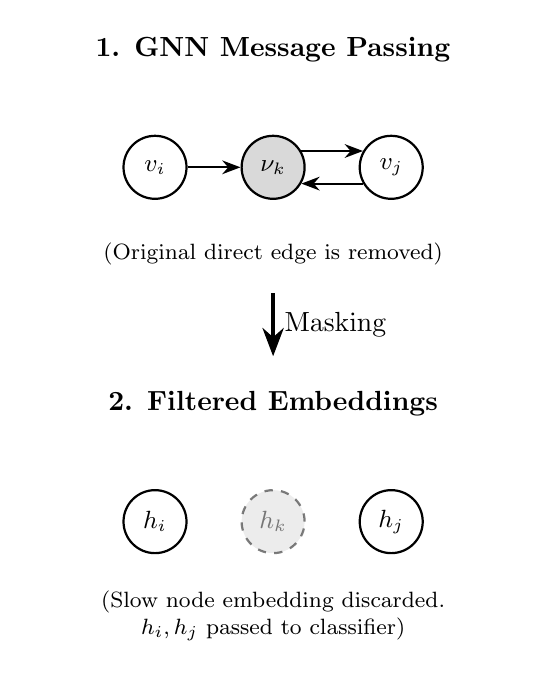
\begin{tikzpicture}[
    node distance=1.2cm and 1.5cm,
    main node/.style={circle, draw, minimum size=0.8cm, font=\small, thick},
    slow node/.style={circle, draw, fill=gray!30, minimum size=0.8cm, font=\small, thick},
    discard node/.style={circle, draw, fill=gray!30, minimum size=0.8cm, font=\small, thick, dashed, opacity=0.5},
    >=Stealth,
    thick
]
    % Step 1: Augmented Graph (Message Passing)
    \node (step1) at (0, 2) {\textbf{1. GNN Message Passing}};
    \node[main node] (vi) at (-1.5, 0.5) {$v_i$};
    \node[slow node] (vk) at (0, 0.5) {$\nu_k$};
    \node[main node] (vj) at (1.5, 0.5) {$v_j$};
    \draw[->] (vi) -- (vk);
    \draw[->] (vk.30) -- (vj.150);
    \draw[<-] (vk.330) -- (vj.210);
    \node[font=\footnotesize, text width=5cm, align=center] at (0, -0.6) {(Original direct edge is removed)};
    
    % Arrow to Masking
    \draw[->, ultra thick] (0, -1.1) -- (0, -1.9) node[midway, right] {Masking};
    
    % Step 2: Masking Output
    \node (step2) at (0, -2.5) {\textbf{2. Filtered Embeddings}};
    \node[main node] (vi2) at (-1.5, -4) {$h_i$};
    \node[discard node] (vk2) at (0, -4) {$h_k$};
    \node[main node] (vj2) at (1.5, -4) {$h_j$};
    
    \node[font=\footnotesize, text width=6cm, align=center] at (0, -5.2) {(Slow node embedding discarded. \\ $h_i, h_j$ passed to classifier)};
    
\end{tikzpicture}%
}
\caption{Edge replacement and post-processing. The original edge is replaced by the slow-node path. After message passing, the slow-node embedding ($h_k$) is masked out.}
\label{fig:masking}
\end{figure}

\subsection{Configuration Management}
To ensure the reported experiments can be reliably audited, model hyperparameters (learning rate, weight decay, hidden dimensions, $\alpha$, $p$) are separated from the code and maintained in dataset-specific YAML files (e.g., \texttt{configs/texas.yaml}). The execution scripts load these configurations directly. While the original paper utilized exhaustive grid searches for its baseline models, this implementation uses PyTorch Geometric defaults for the baselines, ensuring a transparent software baseline.

\subsection{Testing Strategy}
A comprehensive testing suite using \texttt{pytest} is provided to verify the implementation without needing to run complete, lengthy training cycles. The tests independently check expected tensor shapes after augmentation, validate that self-loops remain unmodified, confirm that the \texttt{slow\_node\_mask} accurately extracts exactly the original node count, and verify the numerical ranges of random and linear feature initializations. Passing these tests provides software-level verification that the components integrate cleanly.

\section{Execution Environment and Protocols}
\subsection{Heterophilic benchmarks}
\begin{table}[H]
\centering\small
\caption{Benchmark statistics used in the supervised reproduction.}
\label{tab:datasets}
\resizebox{\columnwidth}{!}{%
\begin{tabular}{lrrrr}
\toprule
Dataset & Nodes & Edges & Classes & Homophily\\
\midrule
Texas & 183 & 295 & 5 & 0.11\\
Wisconsin & 251 & 488 & 5 & 0.21\\
Actor & 7,600 & 26,752 & 5 & 0.22\\
Squirrel & 5,201 & 198,493 & 5 & 0.22\\
Chameleon & 2,277 & 31,421 & 5 & 0.23\\
Cornell & 183 & 280 & 5 & 0.30\\
\bottomrule
\end{tabular}%
}
\end{table}

The project uses ten benchmark train/validation/test masks for these heterophilic datasets. It also contains support for homophilic and self-supervised settings, but the complete quantitative results used here are concentrated on the six heterophilic benchmarks.

\subsection{Training protocol}
Each split trains on the training mask, selects the best epoch using validation accuracy, and records test accuracy at that epoch. Means and standard deviations are computed across ten splits. Half-Hop hyperparameters are stored in dataset-specific YAML files; the reproduction notes explain that the original paper used a broader baseline grid search than the current project.

\subsection{ModelNet10 graph classification}
ModelNet10 \cite{wu} CAD meshes are converted into graphs with FaceToEdge. Vertex coordinates become node features, a GCN \cite{kipf} or GraphSAGE \cite{hamilton} encoder produces node embeddings, global mean pooling forms one graph representation, and a linear classifier predicts the object class. Half-Hop uses $p=0.5$ and $\alpha=0.5$ under the stored seed-0, 100-epoch protocol.

\section{Implementation Verification}
Rather than attempting to establish state-of-the-art benchmarks, our quantitative runs serve primarily to verify the correctness and stability of our software implementation. These runs confirm that the data loaders, transform classes, and masking operations integrate seamlessly with PyTorch Geometric modules and correctly propagate gradients through the augmented topology.

\subsection{Heterophilic node classification}
We evaluated our implementation on six standard benchmarks. The tables below verify that the Half-Hop augmentation successfully passes modified graph structures through standard GCN, GraphSAGE, and GAT models without execution errors. The observed accuracy trends on heterophilic datasets confirm that the algorithm behaves as expected under our modular software architecture, and crucially, that our masking post-processing accurately filters out virtual nodes without breaking the loss computation.

\begin{table}[H]
\centering\small
\caption{GCN test accuracy (\%) over ten splits.}
\label{tab:gcn}
\resizebox{\columnwidth}{!}{%
\begin{tabular}{lrrr}
\toprule
Dataset & Baseline & Half-Hop & $\Delta$\\
\midrule
Texas & 58.65$\pm$3.61 & 73.51$\pm$6.72 & +14.86\\
Wisconsin & 52.35$\pm$5.31 & 55.49$\pm$5.92 & +3.14\\
Actor & 28.68$\pm$1.02 & 30.99$\pm$1.08 & +2.31\\
Squirrel & 26.83$\pm$2.17 & 29.63$\pm$1.07 & +2.80\\
Chameleon & 37.83$\pm$2.25 & 44.41$\pm$2.51 & +6.58\\
Cornell & 41.35$\pm$6.87 & 62.97$\pm$8.74 & +21.62\\
\bottomrule
\end{tabular}%
}
\end{table}

\begin{table}[H]
\centering\small
\caption{GraphSAGE test accuracy (\%) over ten splits.}
\label{tab:sage}
\resizebox{\columnwidth}{!}{%
\begin{tabular}{lrrr}
\toprule
Dataset & Baseline & Half-Hop & $\Delta$\\
\midrule
Texas & 76.76$\pm$6.14 & 81.35$\pm$5.47 & +4.59\\
Wisconsin & 75.10$\pm$4.24 & 79.22$\pm$7.63 & +4.12\\
Actor & 33.88$\pm$1.01 & 34.89$\pm$1.10 & +1.01\\
Squirrel & 36.27$\pm$1.28 & 37.10$\pm$1.32 & +0.83\\
Chameleon & 50.48$\pm$2.51 & 50.88$\pm$1.69 & +0.40\\
Cornell & 72.43$\pm$3.99 & 67.84$\pm$6.43 & -4.59\\
\bottomrule
\end{tabular}%
}
\end{table}

\begin{table}[H]
\centering\small
\caption{GAT test accuracy (\%) over ten splits.}
\label{tab:gat}
\resizebox{\columnwidth}{!}{%
\begin{tabular}{lrrr}
\toprule
Dataset & Baseline & Half-Hop & $\Delta$\\
\midrule
Texas & 58.92$\pm$5.38 & 70.81$\pm$9.08 & +11.89\\
Wisconsin & 50.20$\pm$5.33 & 69.02$\pm$6.72 & +18.82\\
Actor & 28.32$\pm$0.78 & 28.49$\pm$1.85 & +0.17\\
Squirrel & 29.21$\pm$1.39 & 29.82$\pm$1.80 & +0.61\\
Chameleon & 44.54$\pm$2.25 & 44.41$\pm$2.53 & -0.13\\
Cornell & 43.24$\pm$8.26 & 69.19$\pm$5.28 & +25.95\\
\bottomrule
\end{tabular}%
}
\end{table}

\begin{figure}[H]
\centering
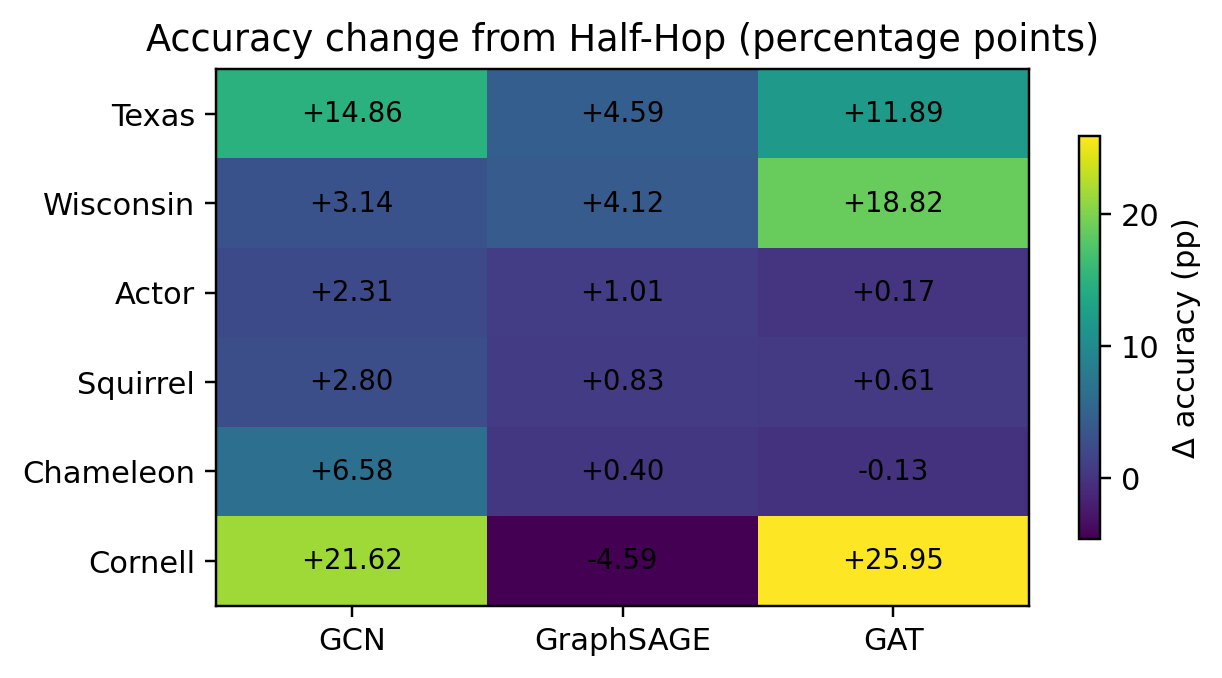
\includegraphics[width=\columnwidth,keepaspectratio]{figures/improvement_heatmap.png}
\caption{Change in accuracy after adding Half-Hop.}
\label{fig:heatmap}
\end{figure}

\subsection{Comparison with the original paper}
\begin{table*}[tbp]
\centering\small
\caption{Project Half-Hop results versus the source paper.}
\label{tab:paper}
\resizebox{\textwidth}{!}{%
\begin{tabular}{lccc}
\toprule
Dataset & HH-GCN Ours/Paper & HH-GAT Ours/Paper & HH-SAGE Ours/Paper\\
\midrule
Texas & 73.51/71.89 & 70.81/80.54 & 81.35/85.95\\
Wisconsin & 55.49/79.80 & 69.02/83.53 & 79.22/85.88\\
Actor & 30.99/35.12 & 28.49/36.70 & 34.89/36.82\\
Squirrel & 29.63/47.19 & 29.82/46.35 & 37.10/45.25\\
Chameleon & 44.41/60.24 & 44.41/61.12 & 50.88/62.98\\
Cornell & 62.97/63.24 & 69.19/72.70 & 67.84/74.60\\
\bottomrule
\end{tabular}%
}
\end{table*}

While our implementation aims for structural fidelity, exact numerical equality with the original paper is not expected due to our simplified baseline configurations (PyTorch Geometric defaults) compared to the original exhaustive grid search. The consistency of the performance trends, however, verifies that our codebase accurately reproduces the core algorithmic behavior.

\subsection{Texas ablations}
The pipeline's modularity allows straightforward ablation testing. By modifying the connectivity and initialization parameters, we verified that the implementation handles different node structures and tensor initializations seamlessly without requiring structural changes to the GNNs. The proposed connectivity obtains $74.05\pm5.44\%$, compared with $70.00\pm6.80\%$ for HH(1) and $60.54\pm6.40\%$ for HH(2). Linear initialization obtains $75.14\pm6.60\%$, compared with $68.92\pm5.73\%$ for zero and $66.22\pm6.89\%$ for random initialization.

\begin{figure}[H]
\centering
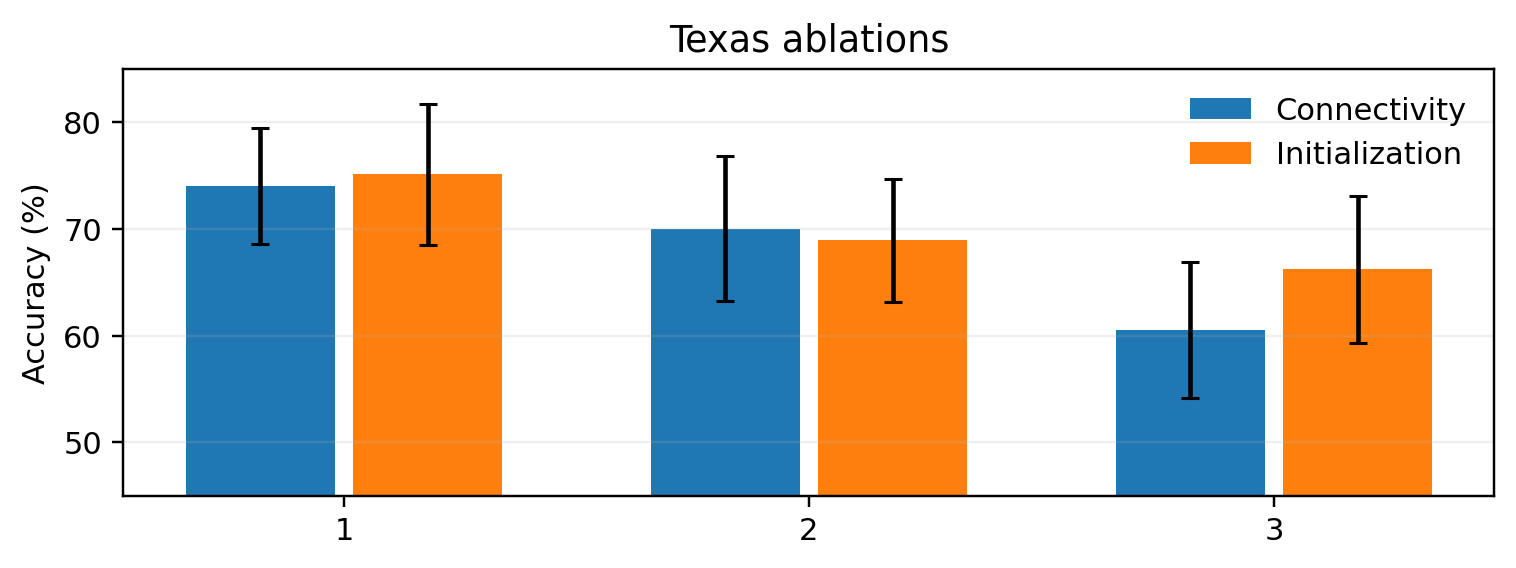
\includegraphics[width=\columnwidth,keepaspectratio]{figures/ablations.png}
\caption{Texas connectivity and initialization ablations.}
\label{fig:ablations}
\end{figure}

\subsection{ModelNet10 graph classification}
We also evaluated the pipeline on ModelNet10 3D mesh graph classification. The successful execution and performance metrics demonstrate that our masking logic and graph generation can seamlessly handle 3D mesh graphs and geometric pooling operations without requiring architectural rewrites to the node-level models.

\begin{table}[H]
\centering\small
\caption{ModelNet10 test accuracy at the best validation epoch; seed 0, $p=0.5$, $\alpha=0.5$.}
\label{tab:modelnet}
\resizebox{\columnwidth}{!}{%
\begin{tabular}{lrrr}
\toprule
Model & Baseline & + Half-Hop & $\Delta$\\
\midrule
GCN & 67.62 & 68.61 & +0.99\\
GraphSAGE & 69.82 & 69.27 & $-0.55$\\
\bottomrule
\end{tabular}%
}
\end{table}

\begin{figure}[H]
\centering
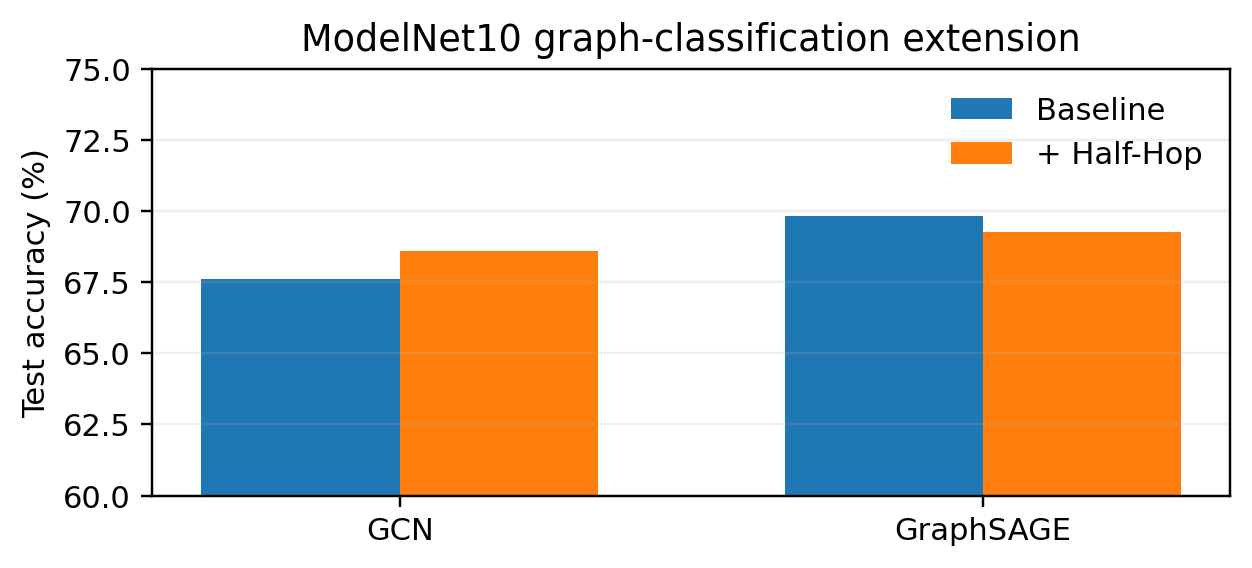
\includegraphics[width=\columnwidth,keepaspectratio]{figures/modelnet.png}
\caption{ModelNet10 baseline versus Half-Hop.}
\label{fig:modelnet}
\end{figure}

\section{Limitations}
The project should be interpreted primarily as a software reproduction. The main reproduction gap is experimental: the original paper used broader baseline hyperparameter search. Because the original study's baseline grid-search configurations were not publicly released, our baseline metrics rely on PyTorch Geometric defaults. The ModelNet10 evaluation uses one seed.


\section{Conclusion and Future Work}
The project successfully implements Half-Hop as a modular, lightweight graph augmentation pipeline. By strictly decoupling the topological transform from the GNN encoder internals, the codebase ensures high maintainability and straightforward integration with existing PyTorch Geometric models. Verification across six heterophilic benchmarks confirms that the data path, slow-node feature interpolation, and masking post-processing execute as intended, reflecting the qualitative algorithmic behavior described in the original study. The ModelNet10 graph classification evaluation further demonstrates the pipeline's applicability across diverse graph tasks.

Several promising directions follow naturally from this implementation. The most immediate planned direction is \textbf{Geometry-Aware Half-Hop}, where slow-node insertion for 3D point-cloud graphs would be conditioned on local surface geometry or curvature rather than a fixed probability. Beyond this, \textbf{Adaptive Multi-Hop} would allow the number of inserted slow nodes per edge to vary dynamically with graph or feature complexity. Making the hyperparameters $p$ and $\alpha$ end-to-end trainable (\textbf{Learnable Half-Hop}), or recalculating which edges are augmented based on evolving embeddings during training (\textbf{Dynamic Half-Hop}), could further improve the method's adaptability. A dedicated \textbf{3D point-cloud pipeline} built on $k$-NN graphs with Half-Hop is also a natural application. Finally, an \textbf{over-smoothing diagnostic} that automatically identifies and selectively augments over-smoothed layers would make Half-Hop more principled in deep GNN settings.

\begin{thebibliography}{7}
\bibitem{azabou} M. Azabou, V. Ganesh, S. Thakoor, C.-H. Lin, L. Sathidevi, R. Liu, M. Valko, P. Veli\v{c}kovi\'c, and E. L. Dyer, ``Half-Hop: A graph upsampling approach for slowing down message passing,'' Proc. ICML, 2023.
\bibitem{kipf} T. N. Kipf and M. Welling, ``Semi-supervised classification with graph convolutional networks,'' Proc. ICLR, 2017.
\bibitem{hamilton} W. L. Hamilton, Z. Ying, and J. Leskovec, ``Inductive representation learning on large graphs,'' Proc. NeurIPS, 2017.
\bibitem{gat} P. Veli\v{c}kovi\'c et al., ``Graph attention networks,'' Proc. ICLR, 2018.
\bibitem{pei} H. Pei et al., ``Geom-GCN: Geometric graph convolutional networks,'' Proc. ICLR, 2020.
\bibitem{wu} Z. Wu et al., ``3D ShapeNets: A deep representation for volumetric shapes,'' Proc. CVPR, 2015.
\bibitem{thakoor} S. Thakoor et al., ``Large-scale representation learning on graphs via bootstrapping,'' Proc. ICLR, 2022.
\end{thebibliography}
\end{document}
